
\chapter{公式、图表和插图}
\label{chap:eqnFigAndTab}
公式、图表和插图广泛使用于学位论文中,并且在正文内存在较多的交叉引用,对他们的高效处理也是\LaTeX{}的优势之一。公式、图表和插图在定义时的共同特点包含:定义中需要设定引用标签、设置图表名称。定义时,图表摆放位置并无要求,\LaTeX{}会根据文稿内容自动计算图表摆放位置,不会出现表格窜行的问题。

\section{公式及术语表}
\label{sec:eqn}

公式定义的内容包含在\textbackslash begin\{equation\}和\textbackslash end\{equation\}之间。为方便,公式的编辑可以采用在线的\LaTeX{}公式编辑器。公式的编号格式可以在./sty文件夹下的格式文件中定义,公式中涉及的术语表也需要在公式后面进行对应标记。

{\bf{推荐公式编辑器:}}http://www.codecogs.com/latex/eqneditor.php?lang=zh-cn 或者 winEdt

{\bf{实例1:}} 以下是L-B非稳态流动升力模型,公式采用在线编辑器编辑,公式后附加有术语说明,公式引用格式为~\ref{eqn:LBmodel},公式后附有术语列表,如\textbackslash nomenclature\{$t$\}\{时间\}。
\begin{equation}
 \label{eqn:LBmodel}
   C_{L}=C_{L0}+C_{L\alpha }\left ( \frac{1+\sqrt{X}}{2} \right )\alpha 
\end{equation}
\nomenclature{$t$}{时间}%
\nomenclature{$\alpha$}{攻角(AoA)}%
\nomenclature{$\dot{\alpha}$}{攻角变化率}%
\nomenclature{$C_{L\alpha}$}{升力线斜率}%
\nomenclature{$C_{L0}$}{$\alpha=0^{\circ}$时当升力}%
\nomenclature{$X$}{相对弦长的非稳态流动分离点}%
\nomenclature{$a_{1}$}{流动分离方程的系数}%
\nomenclature{$\alpha^{\star}$}{$X=0.5$时的攻角}%
\nomenclature{$\tau _{1},\tau _{2}$}{流动分离方程的时间常数}%

\section{表格}
\label{sec:tab}
表格的定义和引用已经在第~\ref{sec:refofFigAndTab}节中介绍,表格内容包含在\textbackslash begin\{table\}和\textbackslash end\{table\}之间,这里只是简单地把\cite{Pattinson:2013_postall_oscillation}文献L-B模型中地变量列表(表~\ref{tab:LB-parameters})显示。

\begin{table}[htb]               % no placement specified: defaults to here, top, bottom, page
\centering
 \begin{center}
  \caption{Physical meaning of parameters in L-B model.}
  \label{tab:LB-parameters}
  \begin{tabular}{cl}
      \toprule
       Parameters & Physical meaning       \\
      \midrule   % \hline
       $C_{L\alpha}$ & Lift curve slope \\
       $a_{1}$ & Controls the shape of the stall curve \\
       $\alpha^{\star}$ & The break point at which $X=0.5$ \\
       $\tau_{1}$ & Represents the tendency of the model to track the static curve \\
       $\tau_{2}$ & Gives the model lift overshoot \\
      \bottomrule
  \end{tabular}
 \end{center}
\end{table}

\section{插图}
\label{sec:fig}

在学位论文中,插图地使用简单地分为两类:单列图片和多列图片。图片地格式包含*.jpg、*.eps、*.pdf,既可以是位图也可以是矢量图,在插入图片是可以定义其高度和宽度。以下实例的实现是建立在引用包subfig和subfigmat的基础上。

{\bf{实例2:}} 单列插入一个jpg或pdf图片:直接在\textbackslash begin\{figure\}和\textbackslash end\{figure\}之间插入\textbackslash includegraphics$\left[width=12cm\right]$\{figName\}即可。

\begin{figure}[htb]
\centering
   \includegraphics[width=12cm]{./img/visual_jpg}
   %\includegraphics[width=6cm,height=5cm]{./img/visual_jpg}
  \caption{插入一个jpg图片}
  \label{fig:visual}
\end{figure}

\begin{figure}[htb]
\centering
   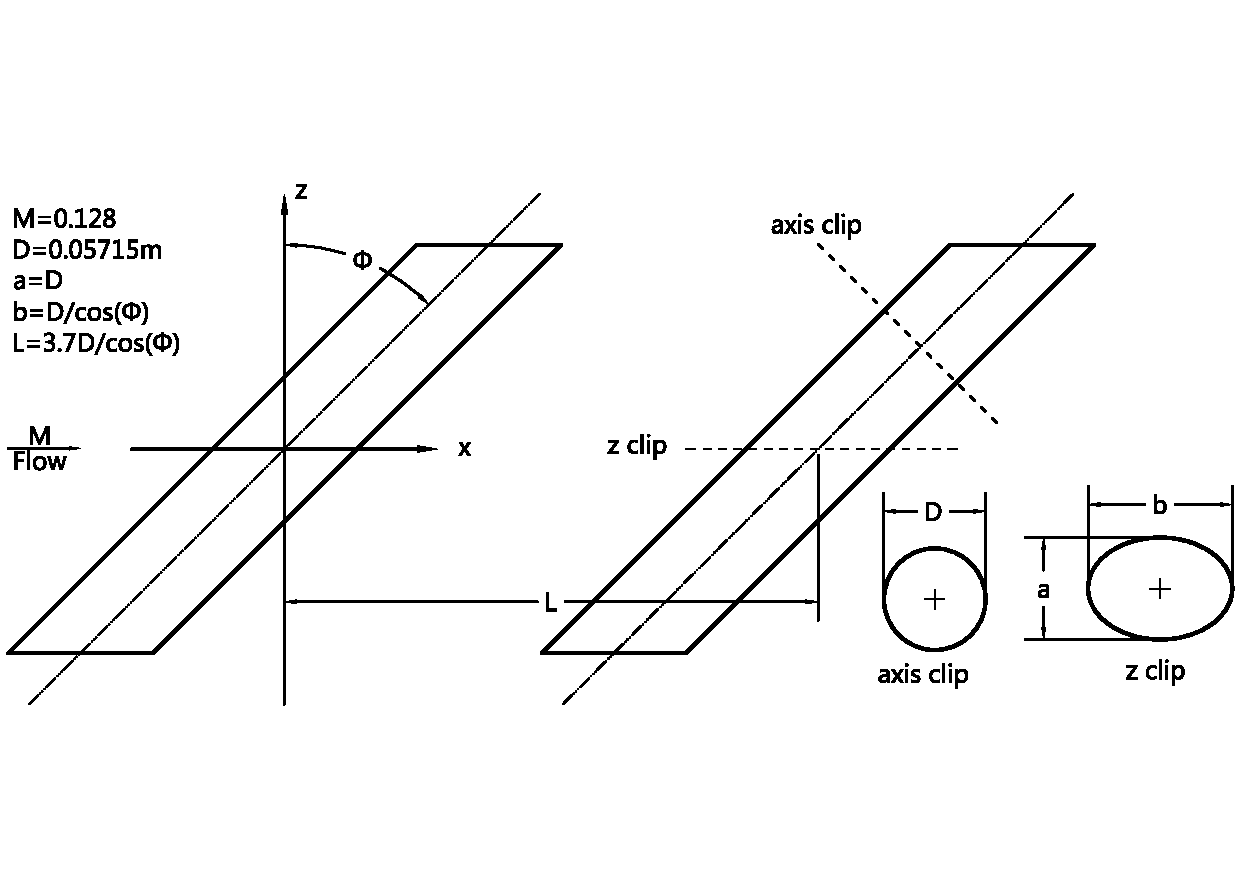
\includegraphics[width=12cm]{./img/Geom_pdf}
  \caption{插入一个pdf图片}
  \label{fig:visual}
\end{figure}

{\bf{实例3:}} 双列插入位图和矢量图:双列的实现依靠\textbackslash begin\{subfigmatrix\}\{2\}和\textbackslash end\{subfigmatrix\},插入图片命令为\textbackslash subfigure。

图片引用是分为单个图片引用和一起引用,例如引用自图片时~\ref{fig:subfig:Curve_jpg},引用全图时~\ref{fig:twoColns}。

% eps 偶尔会有编译问题,且编译速度慢,建议直接用pdf
\begin{figure}[ht!]
    \centering
    \subfigure[jpg位图格式]
    {
        \begin{minipage}{7.0cm}
            \centering
            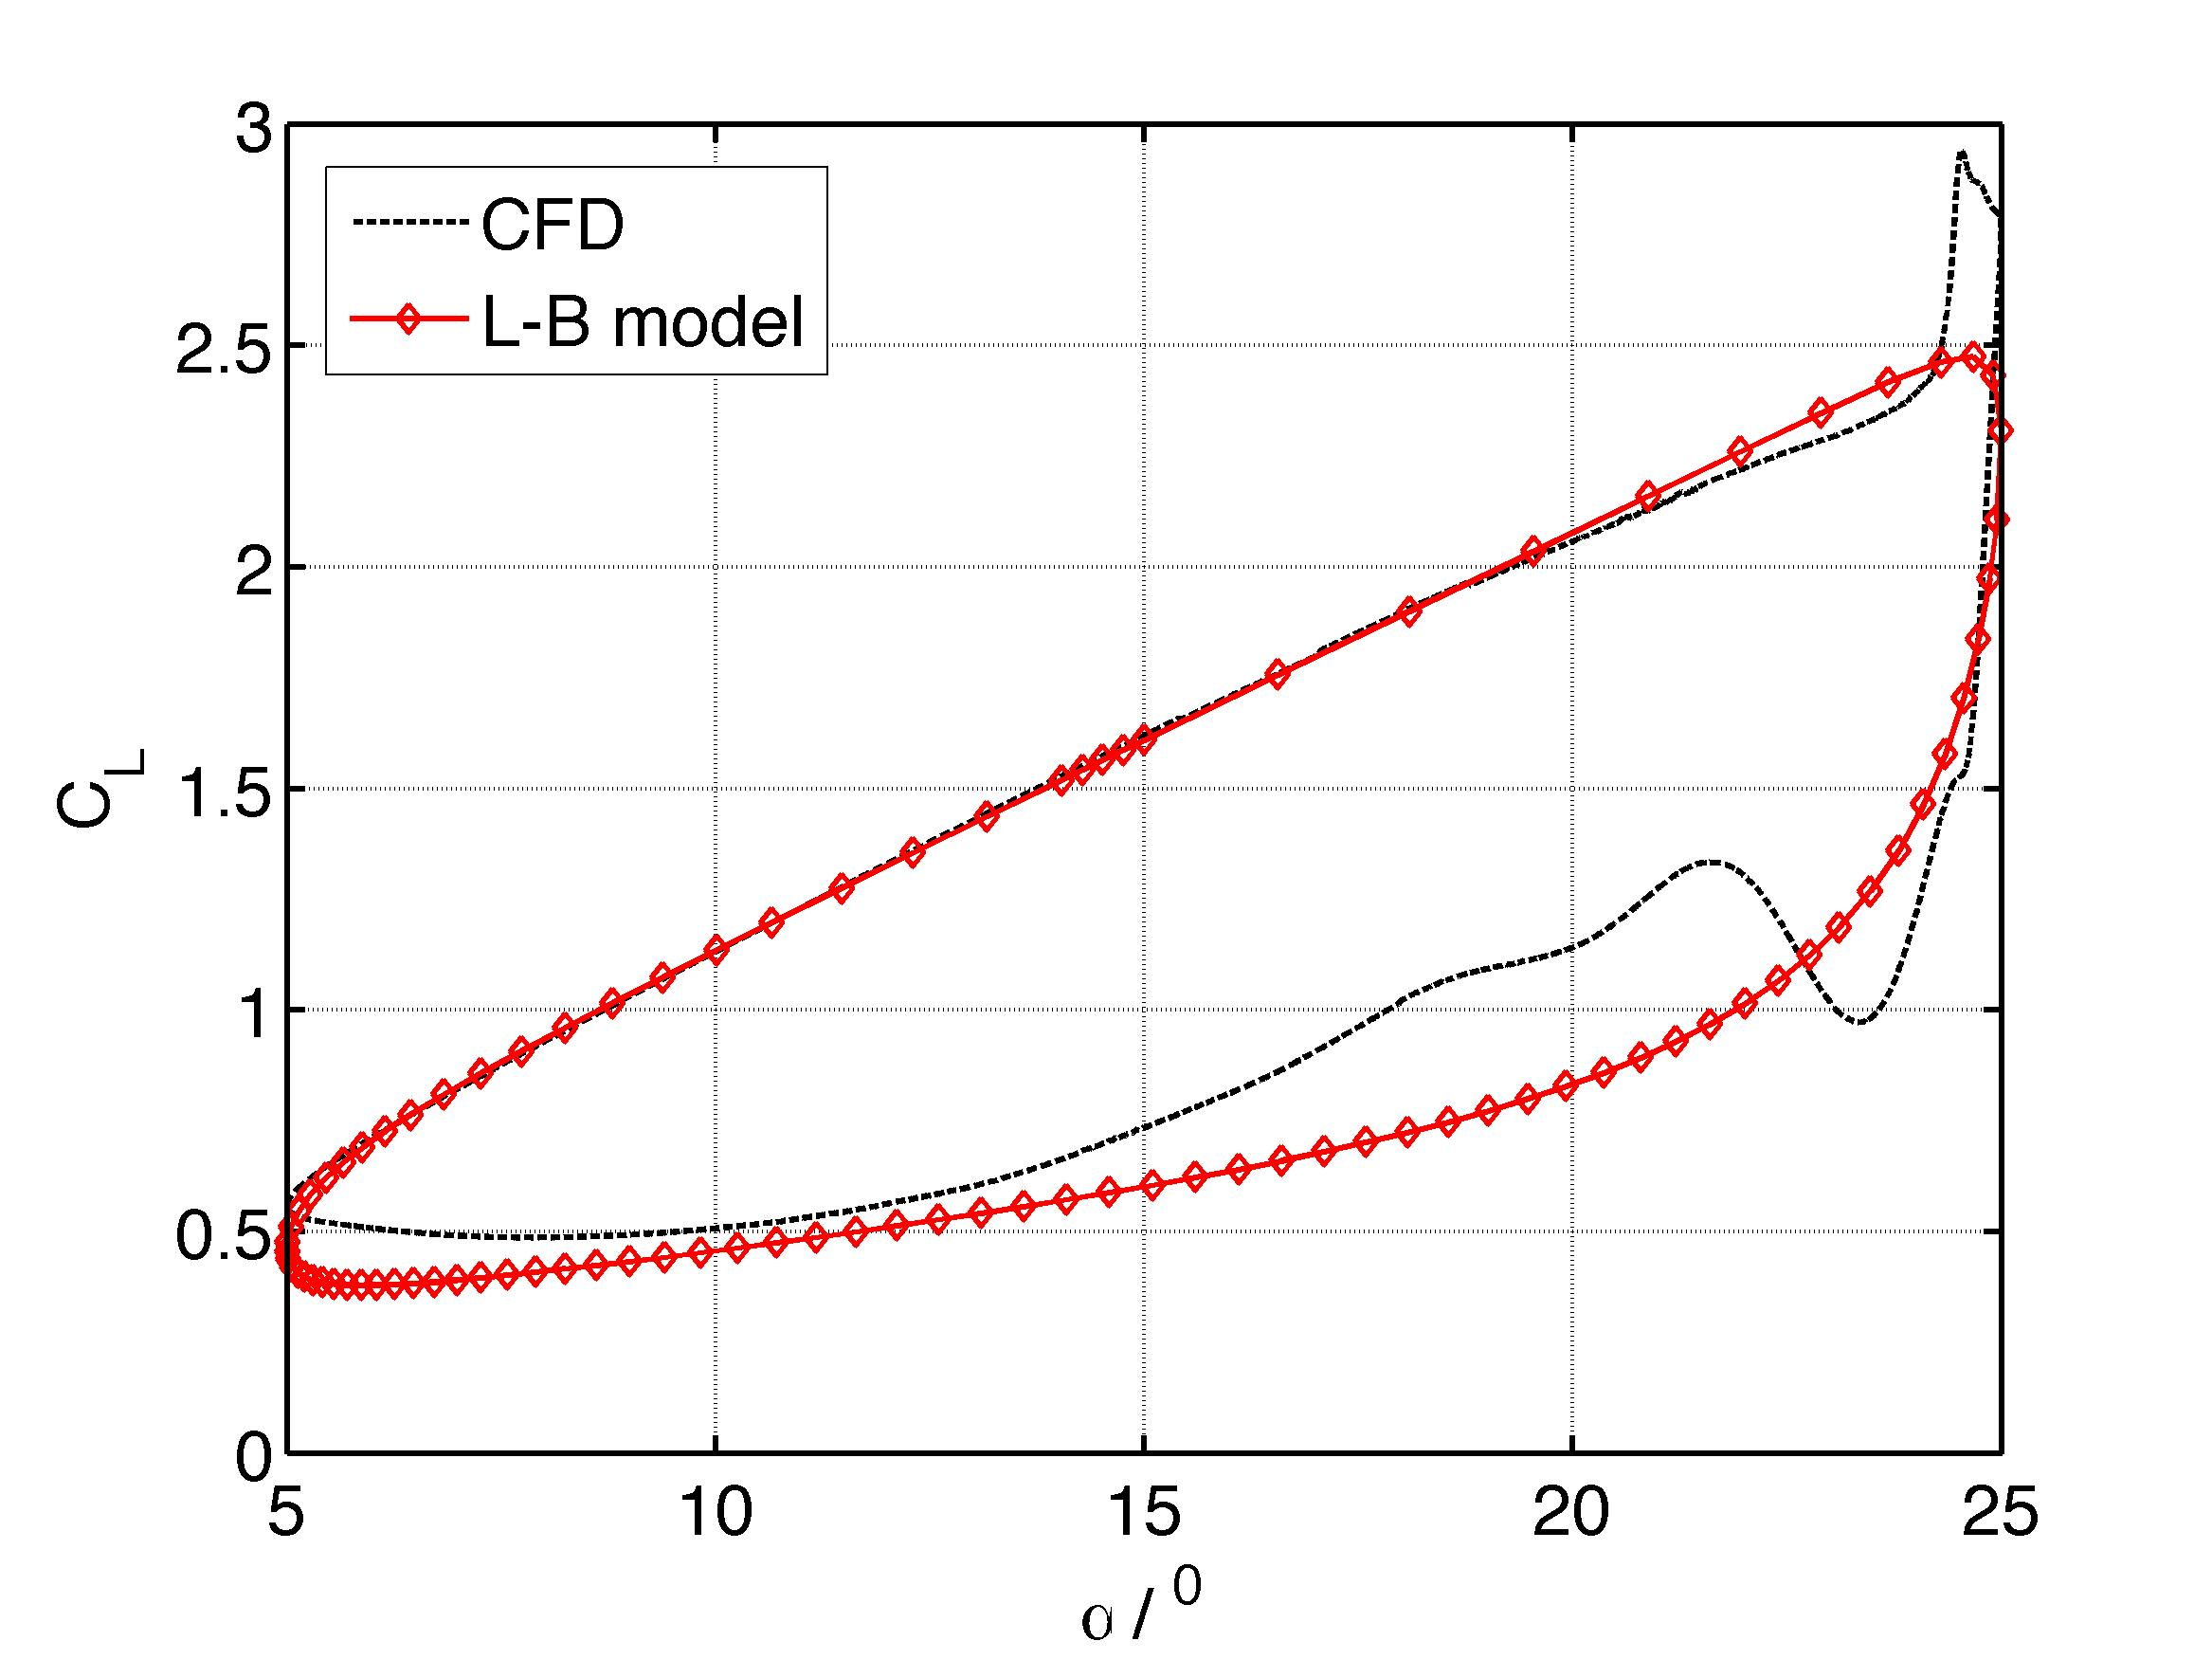
\includegraphics[width=0.9\textwidth]{./img/Curve_jpg}
        \end{minipage}
    \label{fig:subfig:Curve_jpg}}
    \subfigure[eps矢量图格式]
    {
        \begin{minipage}{7.0cm}
            \centering
            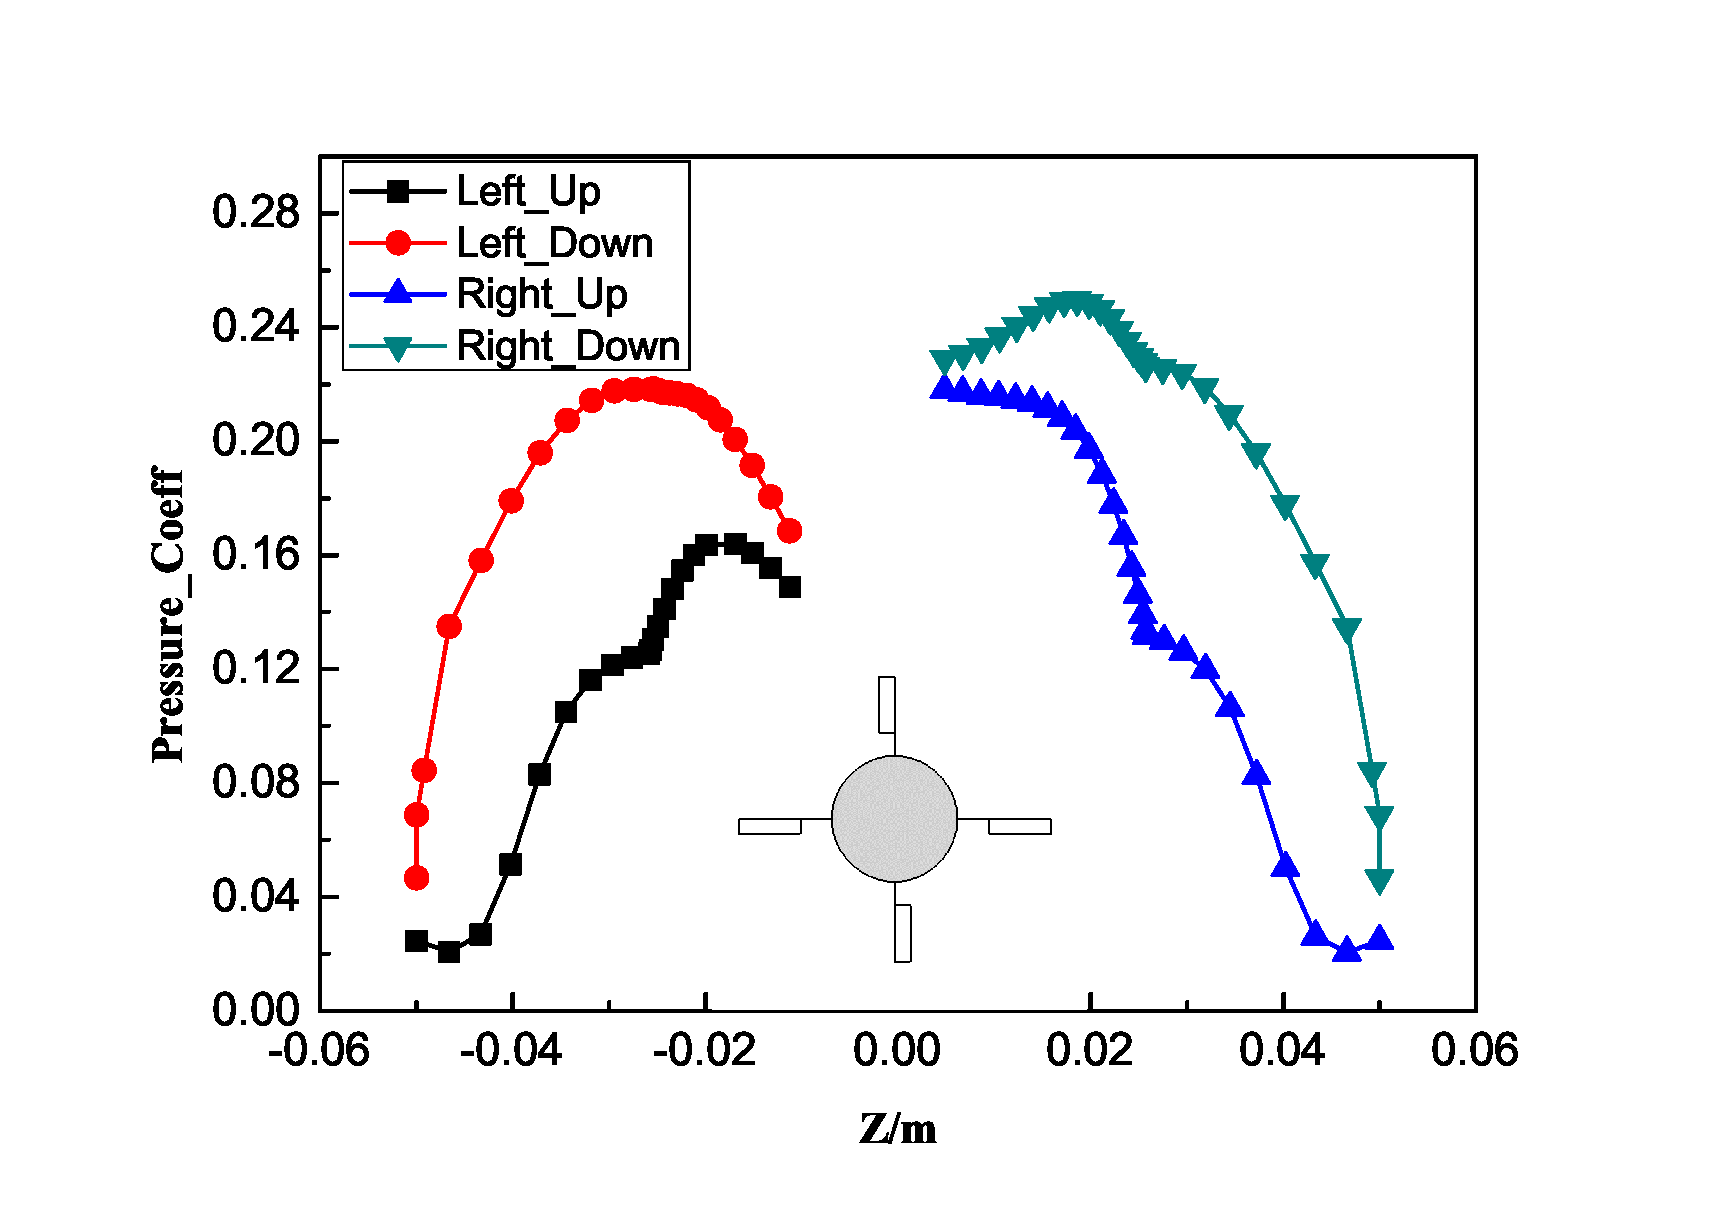
\includegraphics[width=0.9\textwidth]{./img/plot_eps}
        \end{minipage}
    \label{fig:subfig:plot_eps}}
    \caption{插入竖排两列图片:a) jpg位图格式;b) pdf矢量图格式}
    \label{fig:twoColns}
\end{figure}




{\bf{实例4:}} 单行两个图片插入:与实例3不同之处是这里是两个独立的图片,采用{\it\bf{minipage}}方式实现,引用是都是独立的进行引用,如图~\ref{fig:minipage:Curve_jpg}。

\begin{figure}[ht!]
    \centering
    \subfigure[jpg位图格式]
    {
        \begin{minipage}{8.0cm}
            \centering
            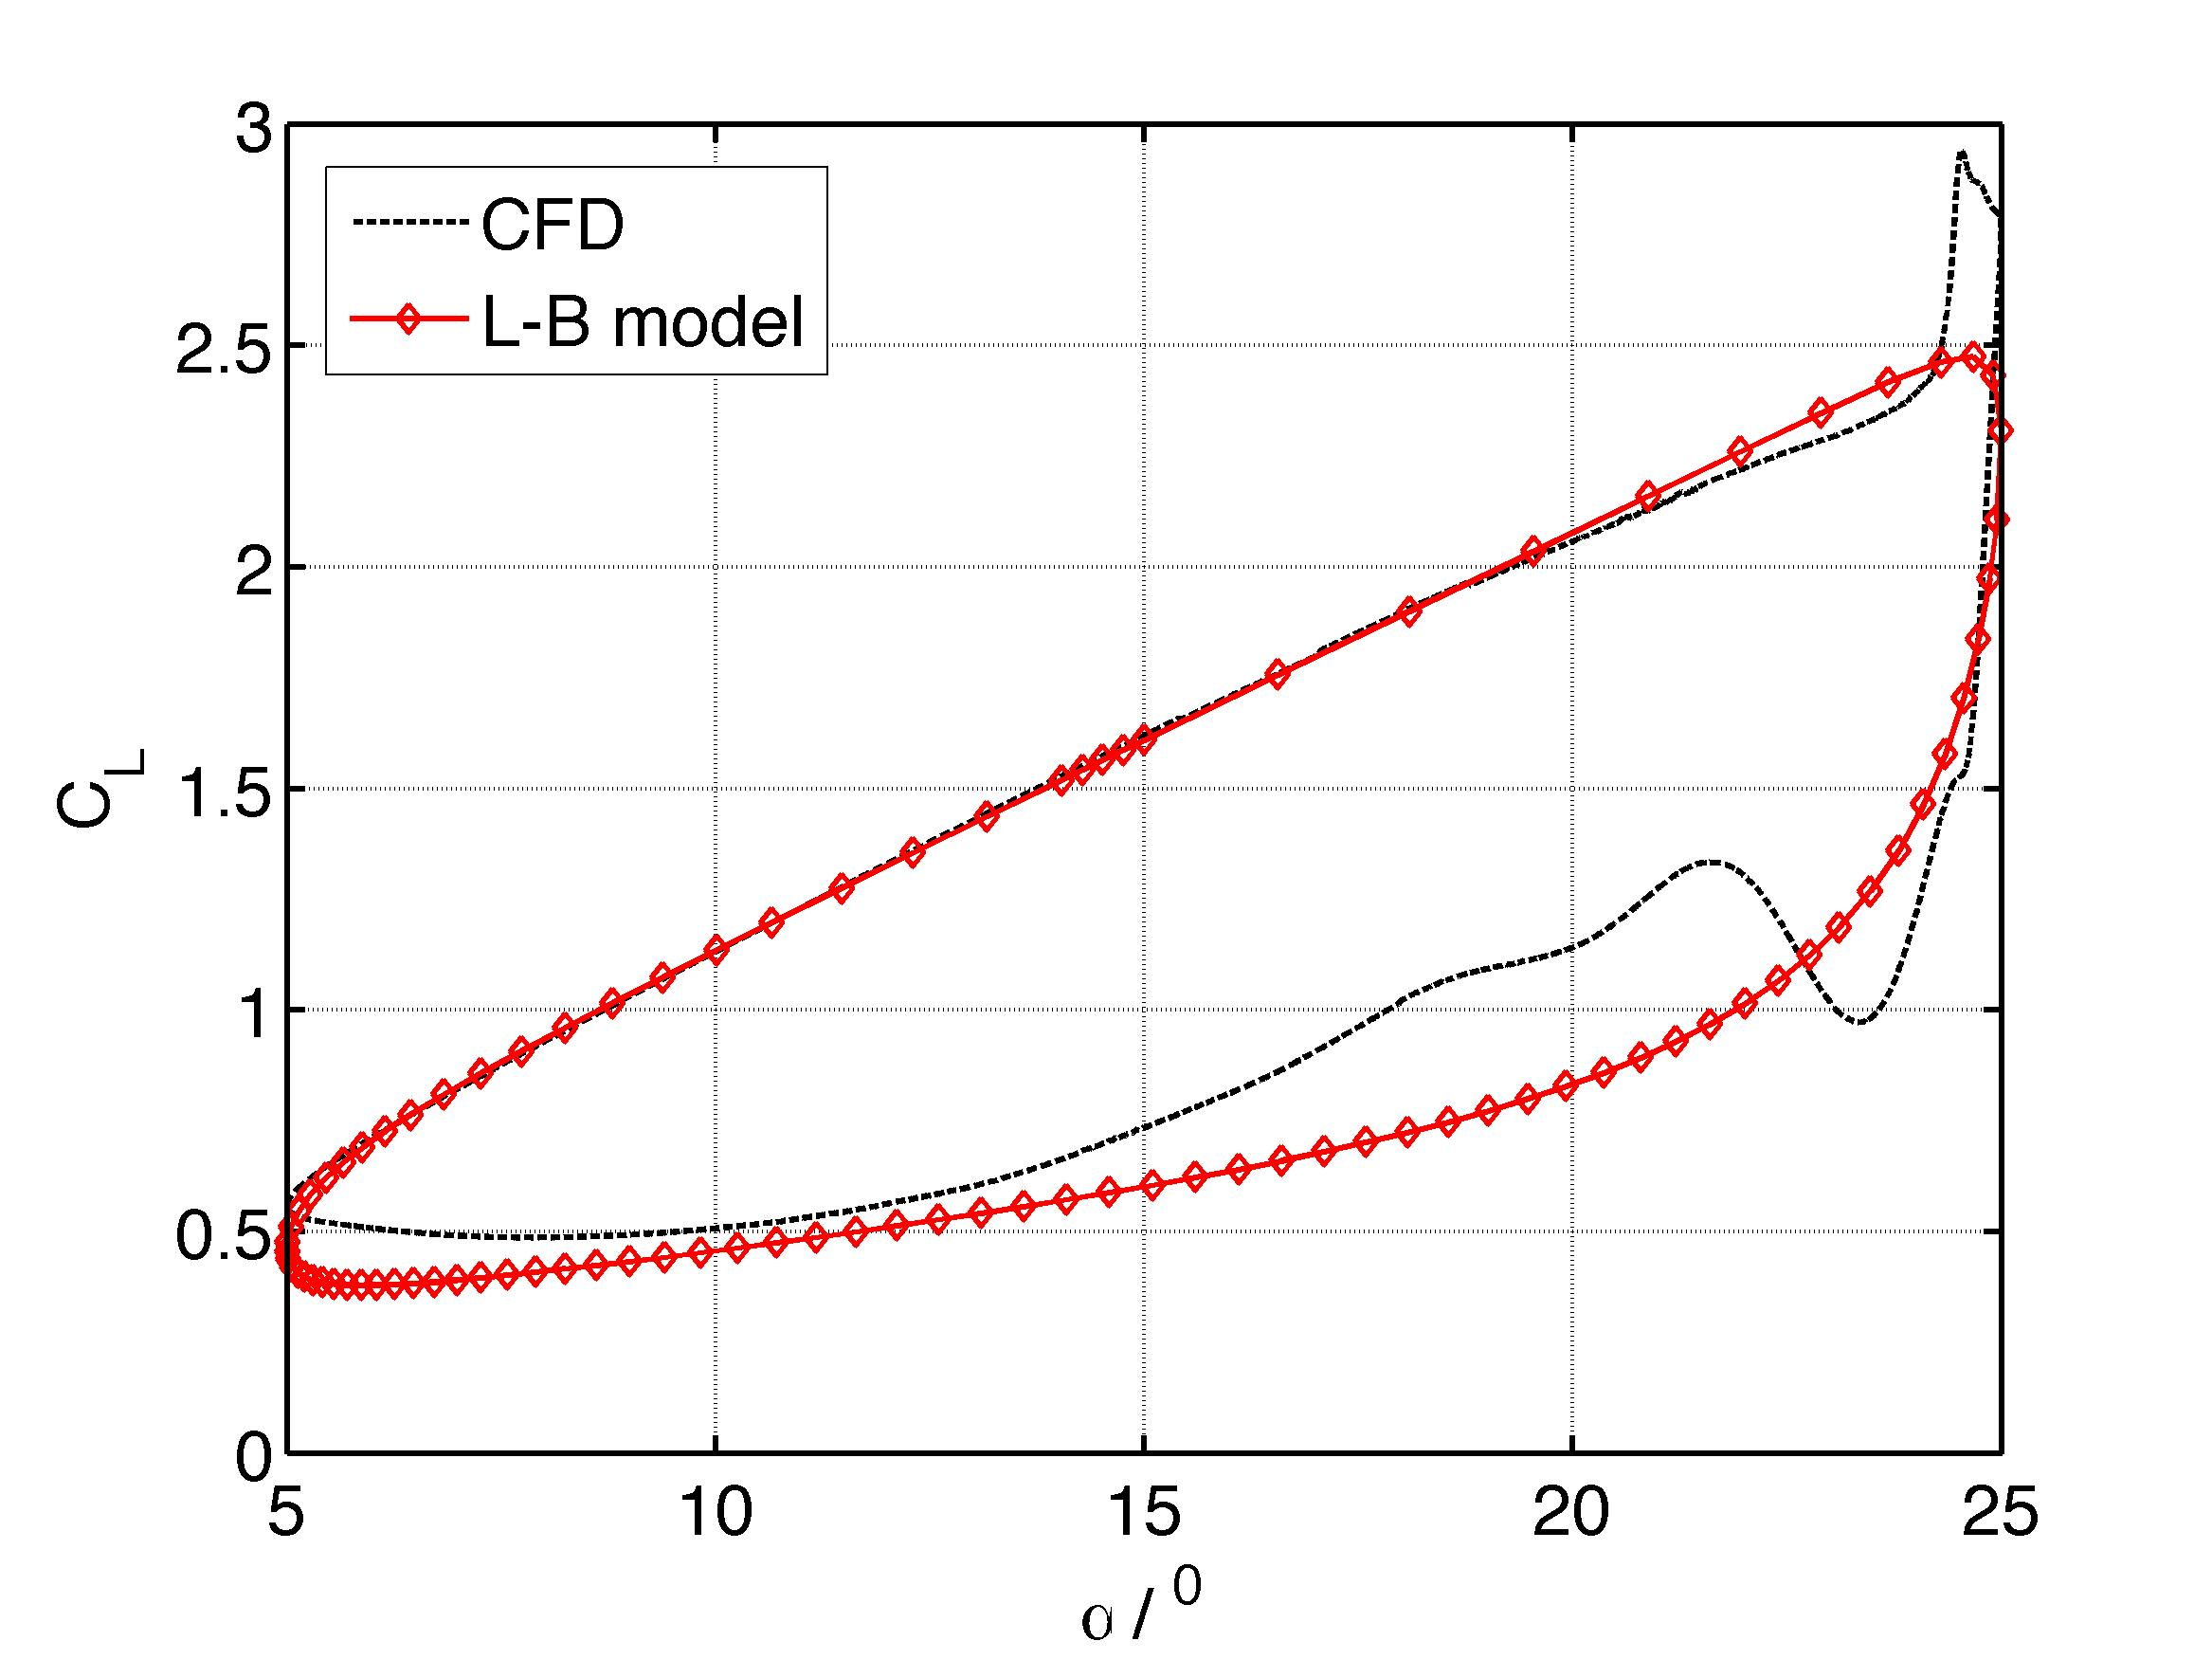
\includegraphics[width=0.9\textwidth]{./img/Curve_jpg}
        \end{minipage}
    \label{fig:minipage:Curve_jpg}}
    \subfigure[eps矢量图格式]
    {
        \begin{minipage}{8.0cm}
            \centering
            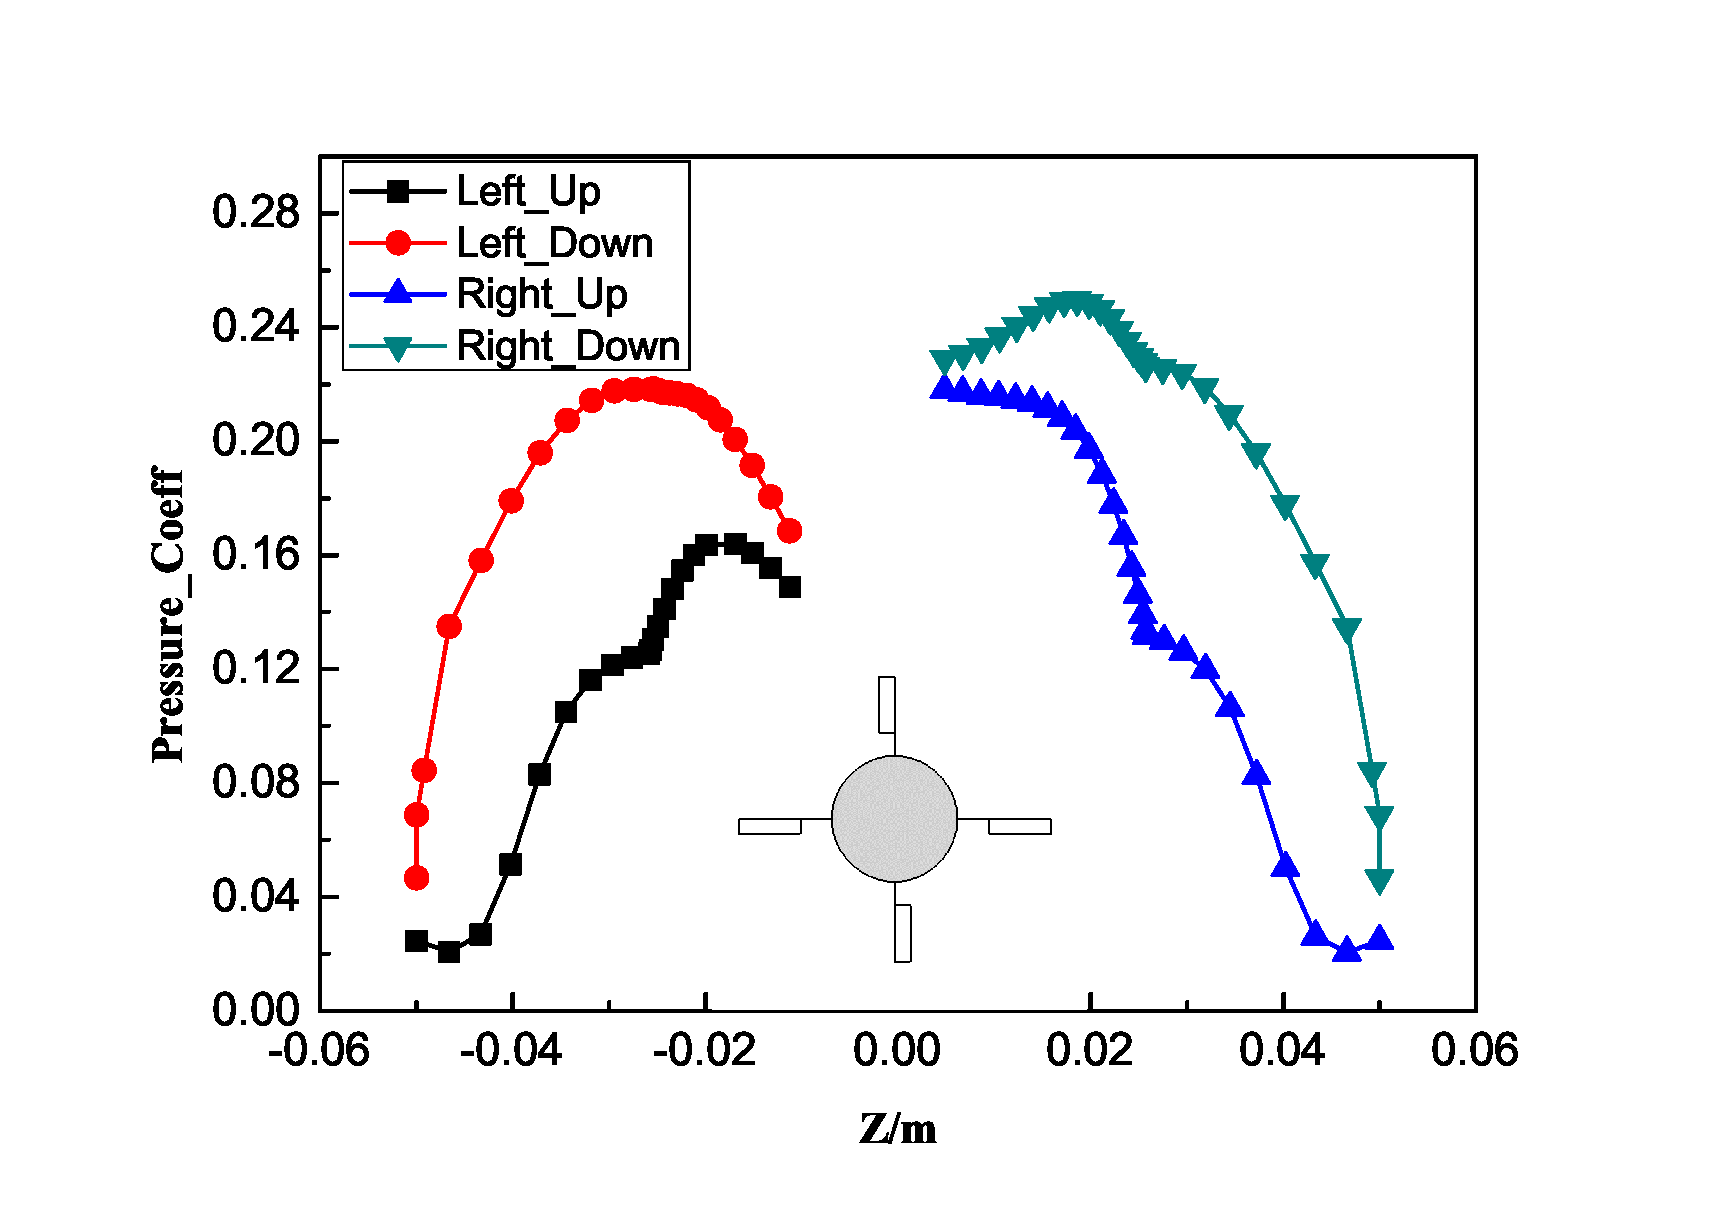
\includegraphics[width=0.9\textwidth]{./img/plot_eps}
        \end{minipage}
    \label{fig:minipage:plot_eps}}
    \caption{插入横排两列图片:a) jpg位图格式;b) eps矢量图格式}
    \label{fig:twoColns}
\end{figure}

{\bf{实例5:}} overpic在图片上进行文字标注:某些时候需要在图片上添加文字说明,并保持原图片格式,这里采用overpic的方法在图片上直接添加文字。

\begin{figure}[htb]
\centering
 \begin{overpic}[width=12cm]{./img/Geom_pdf}
   \put(-8,20){\rotatebox{90}{\footnotesize{纵坐标($r/s$)}}}
   \put(40,2){\footnotesize{手动添加横坐标 ($s$)}}
  \end{overpic}
\caption{在图片上添加文字说明}
\label{fig:overpic}
\end{figure}

尽管可以使用jpg、pdf、eps多种格式的图片,但是这里推荐优先使用eps或pdf的矢量图,提高图片的分辨率。在图片上添加文字说明优先使用overpic的方式,保留原图片。
